\documentclass[10pt]{article}
\usepackage[margin=0.85in]{geometry}
\usepackage{amsmath,amssymb}
\usepackage{graphicx}
\usepackage{booktabs}
\usepackage{algorithm}
\usepackage{algpseudocode}
\usepackage{caption}
\usepackage{float}
\usepackage{tikz}
\usetikzlibrary{positioning,arrows.meta}
\usepackage{microtype}
\usepackage[hidelinks]{hyperref}
\usepackage{enumitem}
\setlist{nosep,leftmargin=*}
\captionsetup{font=small}
\graphicspath{{../figures/}}

\newcommand{\vect}[1]{\mathbf{#1}}
\newcommand{\F}{F_{\mathrm{reg}}}

\title{Surface Registration for Computer Integrated Surgery:\\Closest Points, Rigid ICP and Deformable Registration to a Shape Atlas}
\author{Parmida Mazloomi\\\small Programming Assignments 3, 4 and 5 of JHU EN.601.455/655 Computer Integrated Surgery I (Fall 2025)}
\date{}

\begin{document}
\maketitle
\vspace{-1.5em}

\section{Overview}

A bone has been scanned with CT and its surface segmented into a triangle mesh (1568 vertices, 3135 triangles). In the operating room, an optical tracker follows two rigid bodies with LED markers: body~B is screwed into the bone, and body~A is a pointer whose tip touches points on the bone surface. The goal is the registration $\F$ from bone-body coordinates to CT coordinates, so that the CT model can be used for navigation. The three assignments build this up in steps \cite{handout34,handout5}:
\begin{itemize}
\item \textbf{PA3}: compute the pointer tip $\vect d_k$ in body-B coordinates for each sample, and the closest point $\vect c_k$ on the mesh with $\F=I$; first by brute force, then with a fast spatial search.
\item \textbf{PA4}: iterative closest point (ICP) registration, alternating matching and rigid registration until $\F$ converges.
\item \textbf{PA5}: the bone shape is modelled by a statistical atlas (mean shape plus 6 modes); estimate $\F$ and the mode weights $\lambda_m$ together.
\end{itemize}
The program is written in Python~3.11 with NumPy \cite{numpy} (arrays, \texttt{numpy.linalg.svd} and \texttt{lstsq}, which call LAPACK \cite{lapack}) and Matplotlib \cite{matplotlib} for figures. No registration, closest-point or calibration library code is used.

\section{Mathematical approach}

\paragraph{Frames and the pointer tip.} A frame $F=[R,\vect p]$ maps $\vect x \mapsto R\vect x+\vect p$, with $F_1F_2=[R_1R_2,\,R_1\vect p_2+\vect p_1]$ and $F^{-1}=[R^T,-R^T\vect p]$ \cite{lecframes}. For sample $k$, the poses $F_{A,k}$ and $F_{B,k}$ are found by registering the body-frame marker positions to the measured ones, and \cite{handout34}
\begin{equation}
\vect d_k = F_{B,k}^{-1}\,F_{A,k}\,\vect A_{\mathrm{tip}}, \qquad \vect s_k=\F\,\vect d_k .
\end{equation}

\paragraph{Point-set registration.} For pairs $(\vect a_i,\vect b_i)$ we minimize $\sum_i\|R\vect a_i+\vect p-\vect b_i\|^2$ with the SVD method of Arun et al.\ \cite{arun,lecrigid}. With centred points $\tilde{\vect a}_i=\vect a_i-\bar{\vect a}$, $\tilde{\vect b}_i=\vect b_i-\bar{\vect b}$, form $H=\sum_i\tilde{\vect a}_i\tilde{\vect b}_i^T=USV^T$ and set
\begin{equation}
R = V\,\mathrm{diag}\big(1,1,\det(VU^T)\big)\,U^T,\qquad \vect p=\bar{\vect b}-R\bar{\vect a}.
\end{equation}
Without the diagonal factor, $VU^T$ can be a reflection ($\det=-1$). This happens when the points are coplanar, so that the smallest singular value is zero; flipping the corresponding column of $V$ is then exact, because that column does not affect the fit. With noise it gives the best proper rotation \cite{umeyama}. If two singular values are zero (collinear points), the rotation about the line is undetermined; this cannot occur with the six non-collinear markers used here.

\paragraph{Closest point on a triangle.} Following \cite{lecpairs}, write $\vect a\approx\vect p+\lambda(\vect q-\vect p)+\mu(\vect r-\vect p)$ and solve the $2\times2$ normal equations
\begin{equation}
\begin{bmatrix}\vect e_1\cdot\vect e_1&\vect e_1\cdot\vect e_2\\ \vect e_1\cdot\vect e_2&\vect e_2\cdot\vect e_2\end{bmatrix}
\begin{bmatrix}\lambda\\ \mu\end{bmatrix}=\begin{bmatrix}\vect w\cdot\vect e_1\\ \vect w\cdot\vect e_2\end{bmatrix},\quad \vect e_1=\vect q-\vect p,\ \vect e_2=\vect r-\vect p,\ \vect w=\vect a-\vect p
\end{equation}
by Cramer's rule. If $\lambda,\mu\ge0$ and $\lambda+\mu\le1$, the projection $\vect c=\vect p+\lambda\vect e_1+\mu\vect e_2$ is inside the triangle and is the closest point, since $\vect a-\vect c$ is normal to the plane. Otherwise the closest point lies on an edge. The lecture's table picks one edge from the sign pattern. When two barycentric coordinates are negative the answer can be on either edge that meets at the shared vertex, and in a random test a fixed choice was wrong in 13\% of those cases (obtuse triangles). We therefore project $\vect a$ onto all three edges with
\begin{equation}
\mathrm{ProjectOnSegment}(\vect a,\vect p,\vect q)=\vect p+t^*(\vect q-\vect p),\qquad t^*=\mathrm{clamp}\Big(\tfrac{(\vect a-\vect p)\cdot(\vect q-\vect p)}{\|\vect q-\vect p\|^2},0,1\Big)
\end{equation}
and keep the nearest. This is always correct, and it also handles degenerate triangles, where the $2\times2$ system is singular. The barycentric weights of the result are returned as well, since PA5 needs them.

\paragraph{Bounding-box tree.} Every node of a binary tree holds a group of triangles and the axis-aligned box $[\vect l,\vect u]$ around all their corners. The distance from $\vect a$ to the box, $\|\max(\vect l-\vect a,\vect 0,\vect a-\vect u)\|$, is a lower bound on the distance to any triangle in the node, so if it exceeds the distance $\beta$ to a surface point already found, the node can be skipped \cite{lecpairs}. Since the bound is never larger than the true distance, pruning never removes the true closest point, and the result equals brute force.

\paragraph{Rigid ICP.} ICP minimizes $E(F)=\sum_k \mathrm{dist}(F\vect d_k,\mathcal M)^2$ by alternating (i) matching, $\vect c_k=\arg\min_{\vect c\in\mathcal M}\|F_n\vect d_k-\vect c\|$, and (ii) registration of the pairs $(\vect d_k,\vect c_k)$ \cite{besl,lecreg1}. Each step can only lower $E$, so ICP descends monotonically to a local minimum.

\paragraph{Statistical shape model.} Vertex $v$ of the deformed bone is $\vect m_v(\lambda)=\vect m_{0,v}+\sum_{m=1}^{M}\lambda_m\vect m_{m,v}$ \cite{handout5}; the modes are orthonormal over all 4704 coordinates. If $\vect c_k$ lies on triangle $(s,t,u)$ with barycentric coordinates $(\zeta_k,\xi_k,\psi_k)$, the same barycentric point on the deformed triangle is
\begin{equation}
\vect c_k=\vect q_{0,k}+\sum_m\lambda_m\vect q_{m,k},\qquad \vect q_{m,k}=\zeta_k\vect m_{m,s}+\xi_k\vect m_{m,t}+\psi_k\vect m_{m,u},
\end{equation}
which is linear in $\lambda$ \cite{pa5notes}. With $\F$ and the matches fixed, the weights solve the linear least-squares problem $\min_\lambda\sum_k\|\vect s_k-\vect q_{0,k}-\sum_m\lambda_m\vect q_{m,k}\|^2$.

\paragraph{Linearized combined step.} To update pose and shape together, a small correction $\Delta F=[\Delta R(\boldsymbol\alpha),\boldsymbol\epsilon]$ with $\Delta R\,\vect s\approx\vect s+\boldsymbol\alpha\times\vect s$ is applied to the samples, requiring $\Delta F\vect s_k\approx\vect c_k+\sum_m\Delta\lambda_m\vect q_{m,k}$. Rearranged, this is the handout's equation (7):
\begin{equation}
\vect s_k\times\boldsymbol\alpha-\boldsymbol\epsilon+\sum_m\Delta\lambda_m\vect q_{m,k}\approx\vect s_k-\vect c_k ,
\end{equation}
three rows $[\,\mathrm{skew}(\vect s_k),\,-I,\,\vect q_{1,k}\cdots\vect q_{M,k}\,]$ per sample in the $6+M$ unknowns. Because $\vect c_k$ already includes the current weights, the weight unknowns must be the changes $\Delta\lambda=\lambda^{(t+1)}-\lambda^{(t)}$; the handout writes $\lambda^{(t+1)}$, which would count the current deformation twice. The rotation is then made exact with Rodrigues' formula, $\Delta R=I+\sin\theta\,K+(1-\cos\theta)K^2$ with $\theta=\|\boldsymbol\alpha\|$ and $K=\mathrm{skew}(\boldsymbol\alpha/\theta)$, rather than the non-orthogonal $I+\mathrm{skew}(\boldsymbol\alpha)$.

\section{Algorithmic approach}

\begin{algorithm}[H]
\caption{Batched bounding-box tree search (\texttt{BoundingBoxTree.closest\_points})}
\begin{algorithmic}[1]
\Require query points $\vect a_1\dots\vect a_N$; optional hint triangles (e.g.\ the previous ICP matches)
\State $\beta_k\gets$ distance to the hint triangle, or to the triangles of the leaf reached by always stepping into the nearer child box
\State $P\gets\{(k,\text{root})\}$; $L\gets\emptyset$
\While{$P\neq\emptyset$} \Comment{one tree level per pass, vectorized over all pairs}
  \State keep $(k,n)\in P$ with $\mathrm{dist}(\vect a_k,\mathrm{box}_n)\le\beta_k$
  \State move pairs with leaf $n$ to $L$; replace the others by $(k,\mathrm{left}(n))$ and $(k,\mathrm{right}(n))$
\EndWhile
\State expand $L$ to (query, triangle) pairs; drop those whose triangle box is farther than $\beta_k$
\State test the rest with the closest-point-on-triangle routine; keep the nearest per query
\end{algorithmic}
\end{algorithm}
The tree is built by splitting each node's triangles at the median of their centroids along the longest axis of the centroid spread, until at most 8 triangles remain (1023 nodes, depth 10). For a deforming mesh only the boxes are refit, children before parents. Keeping $\beta_k$ fixed during the walk (instead of lowering it as in the lecture's depth-first search) costs some extra triangle tests but lets each level run as one NumPy operation over all queries.

\begin{algorithm}[H]
\caption{Rigid ICP (\texttt{icp.icp})}
\begin{algorithmic}[1]
\Require tips $\vect d_k$, search structure, $F_0=I$; options: warm-up 3, scale 3, floor 0.5\,mm, tolerance $\tau=10^{-5}$\,mm
\State $\vect s_k\gets F_0\vect d_k$; match $\vect c_k$; $\eta\gets\infty$
\For{$n=1,2,\dots,500$}
  \State \textbf{if} $n>3$: $\eta\gets\max(0.5,\ \min(\eta,\ 3\,\mathrm{mean}_k\|\vect s_k-\vect c_k\|))$ \Comment{shrinking threshold}
  \State inliers $\gets\{k:\|\vect s_k-\vect c_k\|\le\eta\}$, widened if needed to keep at least half the pairs
  \State $F_n\gets$ \textsc{Register}$(\{\vect d_k\},\{\vect c_k\})$ over the inliers; $\vect s_k\gets F_n\vect d_k$; rematch, seeded with the previous triangles
  \State \textbf{stop if} $\max_k\|F_n\vect d_k-F_{n-1}\vect d_k\|<\tau$, or the mean residual changed by less than $10^{-9}$ (relative) for 5 iterations
\EndFor
\end{algorithmic}
\end{algorithm}
The motion test bounds the change of both the rotation and the translation of $\F$ in millimetres at the samples, which is easier to interpret than separate tolerances. The threshold follows the lecture's suggestion of about $3\varepsilon_n$ after a few iterations \cite{lecreg1}.

\begin{algorithm}[H]
\caption{Deformable registration (\texttt{deformable.deformable\_registration})}
\begin{algorithmic}[1]
\State $\lambda\gets0$; $\F\gets$ ICP to the mean shape
\For{3 rounds} \Comment{handout's first method}
  \State repeat up to 10 times: match on the current mesh; solve the weight least squares; deform; refit the tree
  \State $\F\gets$ ICP from the current $\F$ with the shape fixed (tolerance $10^{-3}$\,mm)
\EndFor
\Repeat \Comment{handout's second method}
  \State match; solve (7) for $(\boldsymbol\alpha,\boldsymbol\epsilon,\Delta\lambda)$; $\F\gets[\mathrm{Rodrigues}(\boldsymbol\alpha),\boldsymbol\epsilon]\,\F$; $\lambda\gets\lambda+\Delta\lambda$; refit the tree
\Until{the step moves every sample and vertex by less than $10^{-5}$\,mm}
\end{algorithmic}
\end{algorithm}
Running the alternation to convergence took about 250 mode steps and 280 rigid ICP iterations per debug set, because rigid motions and modes move the points in similar directions and separate steps zigzag. The combined step treats them together; either route reaches the same weights to within 0.001.

\section{Overview of program structure}

\begin{figure}[H]
\centering
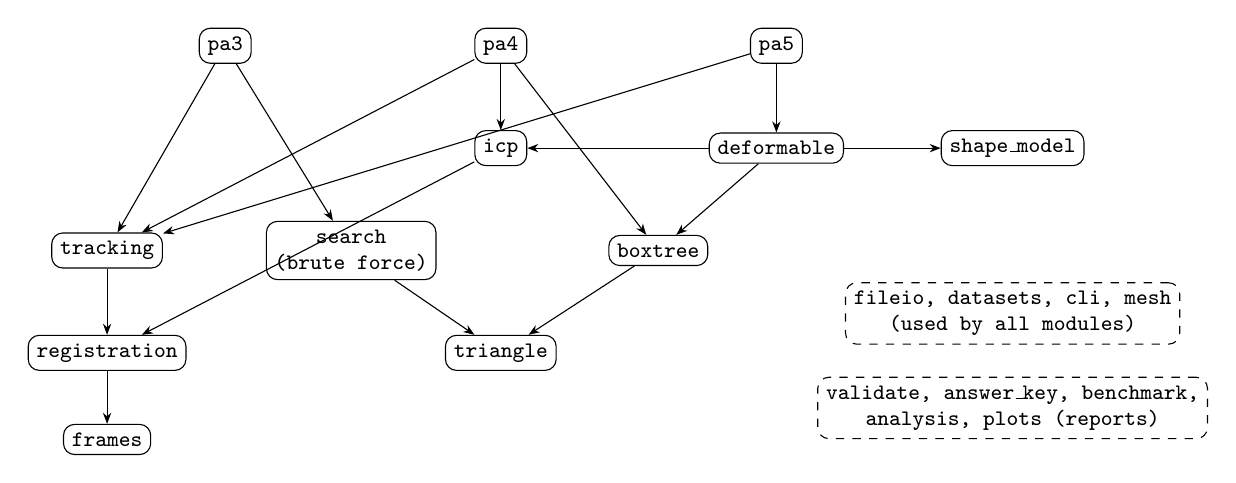
\begin{tikzpicture}[every node/.style={font=\footnotesize\ttfamily, draw, rounded corners, inner sep=3pt, align=center, fill=white}, >={Stealth[length=4pt]}]
\node (pa3) at (0,0) {pa3}; \node (pa4) at (3.5,0) {pa4}; \node (pa5) at (7,0) {pa5};
\node (icp) at (3.5,-1.3) {icp}; \node (def) at (7,-1.3) {deformable}; \node (shape) at (10,-1.3) {shape\_model};
\node (track) at (-1.5,-2.6) {tracking}; \node (search) at (1.6,-2.6) {search\\(brute force)};
\node (tree) at (5.5,-2.6) {boxtree};
\node (reg) at (-1.5,-3.9) {registration}; \node (tri) at (3.5,-3.9) {triangle};
\node (fr) at (-1.5,-5.0) {frames};
\node[dashed] (io) at (10,-3.4) {fileio, datasets, cli, mesh\\(used by all modules)};
\node[dashed] (val) at (10,-4.6) {validate, answer\_key, benchmark,\\analysis, plots (reports)};
\foreach \a/\b in {pa3/track,pa3/search,pa4/icp,pa4/tree,pa4/track,pa5/def,pa5/track,def/icp,def/tree,def/shape,icp/reg,tree/tri,search/tri,track/reg,reg/fr}
  \draw[->] (\a) -- (\b);
\end{tikzpicture}
\caption{Module hierarchy of the \texttt{cisreg} package (arrows: ``uses''). The three programs at the top are the command-line entry points; the dashed boxes are shared input and output code and the tools that produce the validation tables and figures.}
\end{figure}

\begin{table}[H]
\centering\small
\begin{tabular}{@{}lp{0.68\textwidth}@{}}
\toprule
Module & Main functions: inputs $\to$ outputs \\
\midrule
\texttt{fileio} & \texttt{read\_mesh}, \texttt{read\_body}, \texttt{read\_samples}, \texttt{read\_modes}, \texttt{read\_output}, \texttt{read\_logfile}: file $\to$ arrays; \texttt{write\_output}: points, weights $\to$ file in the instructor's layout \\
\texttt{datasets}, \texttt{cli} & file names of each set; \texttt{load\_inputs}: (assignment, set) $\to$ mesh, bodies, readings; shared options \\
\texttt{frames} & \texttt{Frame} (apply, compose, inverse); \texttt{rotation\_from\_vector} (Rodrigues), \texttt{rotation\_angle}, \texttt{frame\_difference} \\
\texttt{registration} & \texttt{register\_points}: paired $(N,3)$ arrays $\to$ \texttt{Frame} (Arun SVD with reflection fix) \\
\texttt{tracking} & \texttt{body\_poses}, \texttt{pointer\_tips}: bodies, readings $\to$ $\vect d_k$ \\
\texttt{triangle} & \texttt{closest\_point\_on\_triangle}: points, corners (broadcast) $\to$ closest points, barycentric weights \\
\texttt{search}, \texttt{boxtree} & \texttt{BruteForceSearch}, \texttt{BoundingBoxTree}: \texttt{closest\_points(queries, hint)} $\to$ points, distances, triangles, weights; \texttt{update\_vertices} \\
\texttt{icp} & \texttt{icp}: $\vect d_k$, search, $F_0$, options $\to$ $\F$, $\vect s_k$, matches, per-iteration history \\
\texttt{shape\_model} & \texttt{ShapeModel.from\_atlas}, \texttt{vertices(}$\lambda$\texttt{)}, \texttt{mesh(}$\lambda$\texttt{)} \\
\texttt{deformable} & \texttt{mode\_basis}, \texttt{solve\_mode\_weights}, \texttt{solve\_combined\_step}, \texttt{deformable\_registration} $\to$ $\F$, $\lambda$, matches, history \\
\texttt{pa3}, \texttt{pa4}, \texttt{pa5} & command-line programs: \texttt{python -m cisreg.pa4 --all} writes \texttt{output/}, logs and summaries \\
\bottomrule
\end{tabular}
\end{table}
Each program writes \texttt{output/PAV-X-Output.txt} in the instructor's format: a header line, for PA5 a line with the mode weights, then $\vect s_k$, $\vect c_k$ and $\|\vect s_k-\vect c_k\|$ per sample.

\section{Validation approach}

\paragraph{Unit tests} (508 tests with pytest, run on every push by GitHub Actions):
\begin{itemize}
\item \emph{Readers}: every file in \texttt{data/} is read and its counts checked against its header.
\item \emph{Registration}: 50 random rigid transforms with 3 to 40 points are recovered to $10^{-9}$; with noise, the estimate fits at least as well as the true frame and no small perturbation improves it; coplanar point sets that make $VU^T$ a reflection are recovered exactly.
\item \emph{Closest point on a triangle}: hand-computed interior, edge and vertex cases above, below and in the plane; collinear and repeated corners; the obtuse two-negative case; and about 800 random point and triangle pairs checked against dense sampling of the triangle.
\item \emph{Tree}: distances identical to brute force for the pointer tips of all 33 data sets, random near and far points, deliberately wrong hints and a deformed mesh; different triangles are accepted only for exact ties at shared edges or vertices.
\item \emph{ICP and PA5}: synthetic surface points with known $\F$ (and weights), with and without noise and injected outliers; the RMS residual never increases without rejection; one combined step recovers a known small correction; mode weights are recovered exactly from exact matches.
\end{itemize}

\paragraph{Debug sets.} Our output files are compared with the instructor's Output and Answer files using $e_{s,k}=\|\vect s_k-\vect s'_k\|$ and $e_{c,k}=\|\vect c_k-\vect c'_k\|$ (max and $\mathrm{RMS}=\sqrt{\mathrm{mean}_k e_k^2}$), and $\max_m|\lambda_m-\lambda'_m|$ for the weights. Since $\vect s_k=\F\vect d_k$, the instructor's $\F$ can be recovered by registering our $\vect d_k$ onto the reference $\vect s'_k$; both frames are then scored by the sum of squared distances to the surface. Full tables are in \texttt{results/pa3\_validation.md}, \texttt{pa4\_validation.md} and \texttt{pa5\_validation.md}.

\paragraph{Rounding floor.} All files are rounded to 0.01\,mm. Two independent roundings give a 3D RMS difference of $\sqrt{3\cdot2\cdot0.01^2/12}=0.0071$\,mm, and a Monte Carlo test (readings perturbed by $\pm0.005$\,mm) shows that the input rounding moves $\vect d_k$ by 0.0073\,mm RMS, about 0.010\,mm in total. This is the level at which two correct programs can agree.

\section{Results}

\paragraph{Debug sets.} Table~\ref{tab:debug} summarizes the agreement. On the noise-free sets everything agrees at the rounding floor. On the noisy PA4 sets our $\vect s_k$ differ from the instructor's by up to 0.05\,mm, but our $\F$ has a lower sum of squared distances (1.578 against 1.602\,mm$^2$ for E, 1.477 against 1.498 for F), so the difference is a different stopping point of the instructor's program, not an error. The noise-free PA5 weights agree to 0.01 to 0.05; perturbing the readings at their rounding level moves them by a standard deviation of 0.014 to 0.041, so the rounded data determine the weights only to that level.

\begin{table}[H]
\centering\footnotesize\setlength{\tabcolsep}{4pt}
\caption{Agreement with the instructor's Output files on the debug and demo sets (mm and degrees).}\label{tab:debug}
\begin{tabular}{@{}lccccc@{}}
\toprule
 & max $e_s$ & RMS $e_s$ & max $e_c$ & $\F$ difference & max weight diff. \\
\midrule
PA3, A to F & 0.010 to 0.022 & 0.008 to 0.011 & 0.014 to 0.020 & ($\F=I$) & \\
PA4, A to D and demos (noise-free) & 0.014 to 0.022 & 0.007 to 0.009 & 0.014 to 0.017 & $\le0.004^\circ$, $\le0.002$ & \\
PA4, E and F (0.1\,mm noise) & 0.051 & 0.021 to 0.024 & 0.045 to 0.051 & $0.02$ to $0.03^\circ$, $\le0.014$ & \\
PA5, A to D (noise-free) & 0.014 to 0.025 & 0.008 to 0.010 & 0.014 to 0.025 & $\le0.0044^\circ$, $\le0.0012$ & 0.011 to 0.046 \\
PA5, E and F (0.1\,mm noise) & 0.028 to 0.033 & 0.012 to 0.014 & 0.025 & $\le0.021^\circ$, $\le0.004$ & 0.20 to 0.34 \\
\bottomrule
\end{tabular}
\end{table}

\begin{figure}[H]
\centering
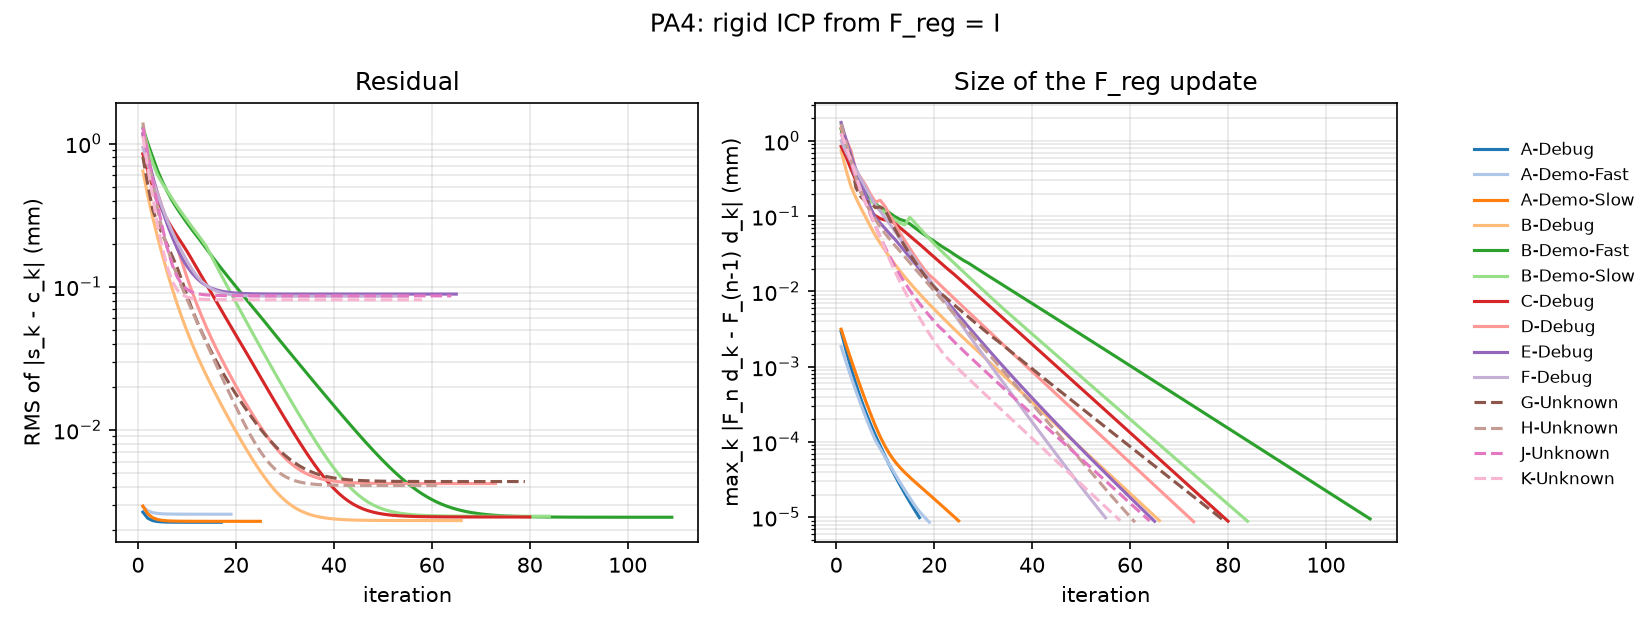
\includegraphics[width=0.49\textwidth]{pa4_convergence.png}\hfill
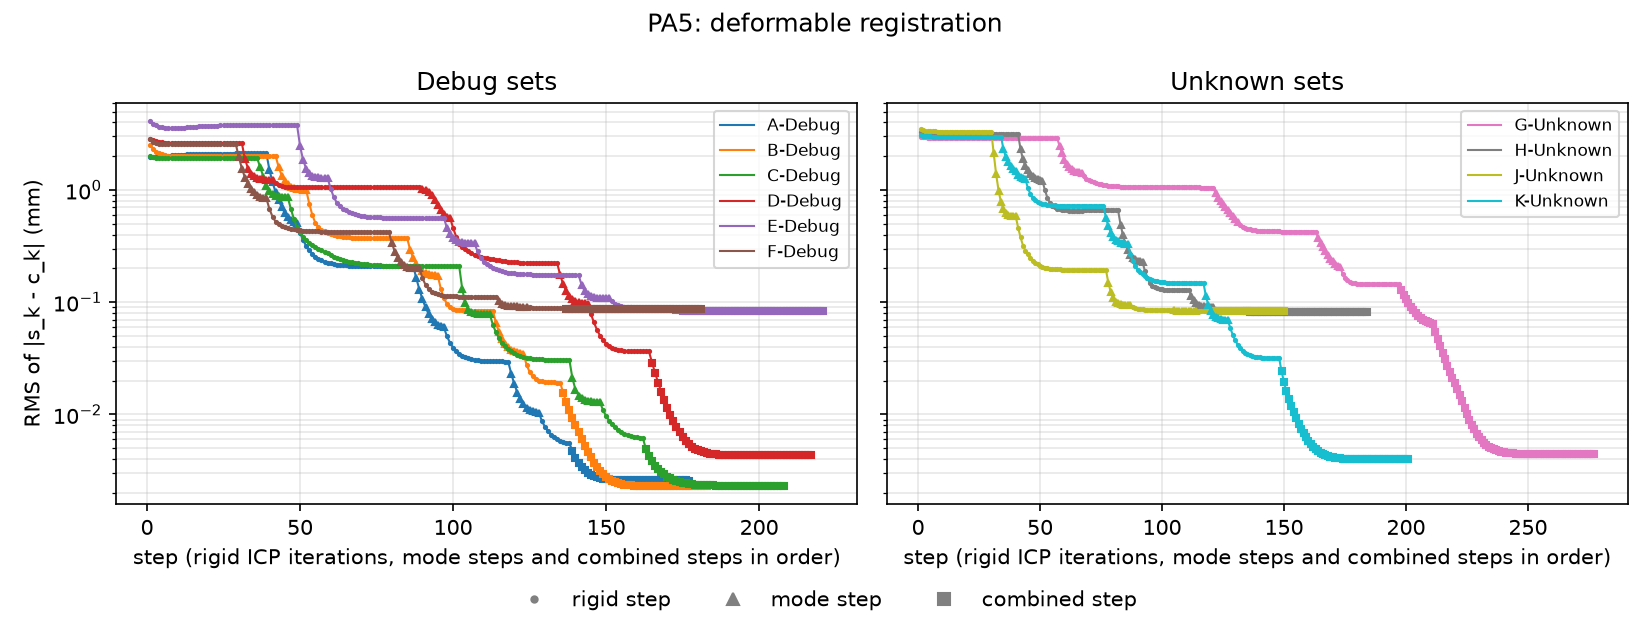
\includegraphics[width=0.49\textwidth]{pa5_convergence.png}
\caption{Left: PA4 RMS residual and size of the $\F$ update per ICP iteration; convergence is linear, to a floor of 0.0025\,mm (noise-free) or 0.085\,mm (noisy). Right: PA5 residual per step. Rigid phases plateau, mode steps (triangles) cause sharp drops, and combined steps (squares) finish.}
\end{figure}

\paragraph{Unknown sets.} Tables~\ref{tab:unk34} and~\ref{tab:unk5} give the results. The outputs were committed before the instructor's log files were opened. A later comparison (\texttt{results/answer\_key\_comparison.md}) found every unknown set registered correctly: within $0.006^\circ$ and 0.003\,mm of the true $\F$ on the noise-free sets and within $0.075^\circ$ and 0.018\,mm on the noisy ones, with errors comparable to the instructor's program. The noise-free PA5 weights are within 0.1 of the true values; with the rounded readings our solution fits the data better than the true parameters do (for example 0.00297 against 0.00360\,mm$^2$ for PA5-G), so the remaining difference is due to the input rounding. The log's ``RMS residual'' turned out to be the mean of $\|\vect s_k-\vect c_k\|$, which is why both are reported.

\begin{table}[H]
\centering\small
\caption{PA3 and PA4 unknown sets. Residuals $\|\vect s_k-\vect c_k\|$ in mm; $\F$ as rotation angle, rotation vector (rad) and translation (mm).}\label{tab:unk34}
\begin{tabular}{@{}llcccccl@{}}
\toprule
Set & N & Iter. & Mean & RMS & Max & Angle & Rotation vector; translation \\
\midrule
PA3-G & 20 & & 1.663 & 1.924 & 3.944 & & $\F=I$ \\
PA3-H & 20 & & 1.538 & 1.700 & 3.010 & & $\F=I$ \\
PA3-J & 20 & & 2.318 & 2.709 & 5.405 & & $\F=I$ \\
PA4-G & 200 & 79 & 0.0033 & 0.0044 & 0.014 & $2.395^\circ$ & $(0.02497, 0.02999, 0.01496)$; $(1.001, -1.500, 0.251)$ \\
PA4-H & 200 & 61 & 0.0033 & 0.0041 & 0.012 & $0.005^\circ$ & $(0.00005, 0.00002, 0.00005)$; $(1.001, 3.001, -2.000)$ \\
PA4-J & 200 & 64 & 0.0667 & 0.0863 & 0.295 & $0.057^\circ$ & $(-0.00026, -0.00040, -0.00086)$; $(3.006, -1.498, 0.505)$ \\
PA4-K & 200 & 58 & 0.0632 & 0.0810 & 0.236 & $0.830^\circ$ & $(0.00881, 0.00478, -0.01045)$; $(-1.489, 2.510, 0.002)$ \\
\bottomrule
\end{tabular}
\end{table}

\begin{table}[H]
\centering\footnotesize\setlength{\tabcolsep}{3.5pt}
\caption{PA5 unknown sets: mode weights, residuals (mm) and $\F$.}\label{tab:unk5}
\begin{tabular}{@{}lcrrrrrrcc@{}}
\toprule
Set & N & $\lambda_1$ & $\lambda_2$ & $\lambda_3$ & $\lambda_4$ & $\lambda_5$ & $\lambda_6$ & Mean / RMS & $\F$ angle; translation \\
\midrule
G & 150 & $-96.381$ & 160.135 & $-81.887$ & $-78.811$ & 126.233 & 141.516 & 0.0036 / 0.0044 & $1.342^\circ$; $(-0.999, 1.001, -1.499)$ \\
H & 400 & 84.172 & 95.279 & $-81.356$ & $-134.684$ & 37.325 & 110.282 & 0.0633 / 0.0813 & $0.036^\circ$; $(1.008, -0.995, 2.003)$ \\
J & 400 & $-5.233$ & $-144.473$ & $-57.066$ & $-132.199$ & 15.544 & $-108.204$ & 0.0647 / 0.0838 & $1.111^\circ$; $(1.495, 1.012, 1.989)$ \\
K & 150 & 54.190 & 153.113 & $-60.647$ & 9.827 & 114.480 & $-43.526$ & 0.0030 / 0.0040 & $0.003^\circ$; $(0.002, 2.000, -0.999)$ \\
\bottomrule
\end{tabular}
\end{table}

\paragraph{Error analysis.} Figure~\ref{fig:analysis} and \texttt{results/error\_analysis.md} summarize four experiments. (i) ICP started from misaligned poses on PA4-B reaches the right minimum in every trial up to $60^\circ$ and 30\,mm, in 92 to 100\% at $75^\circ$, and rarely beyond $120^\circ$; the course data start within $3.5^\circ$ and 6\,mm. (ii) Marker noise propagates linearly: at $\sigma=0.1$\,mm, $\F$ is good to about $0.06^\circ$ and 0.03\,mm, but the PA5 weights only to about 1 unit with 150 samples, so the weights are the least certain output. (iii) The noise-free PA5 sets need all 6 modes; leaving out any mode leaves residuals of 0.3 to 0.9\,mm. (iv) The tree is 2.8 times faster than brute force for one point and 20 to 100 times faster for the 75 to 400 points of a data set, with identical results.

\begin{figure}[H]
\centering
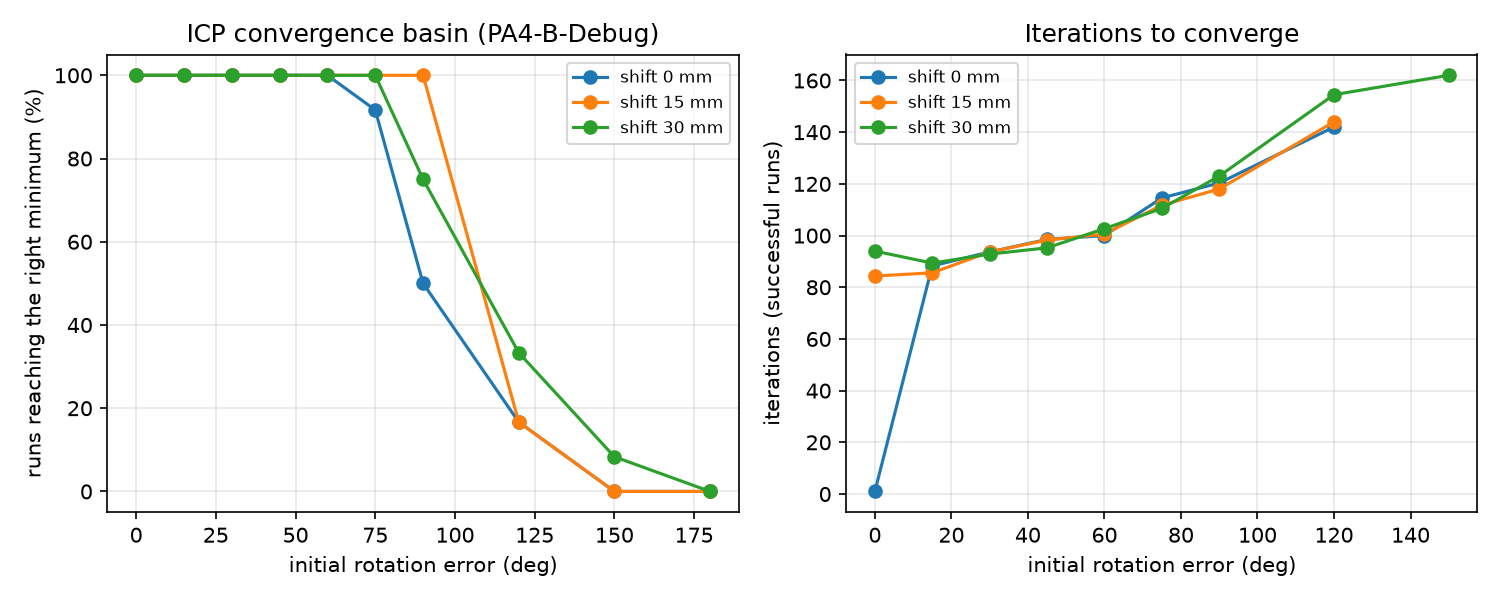
\includegraphics[width=0.49\textwidth]{icp_convergence_basin.png}\hfill
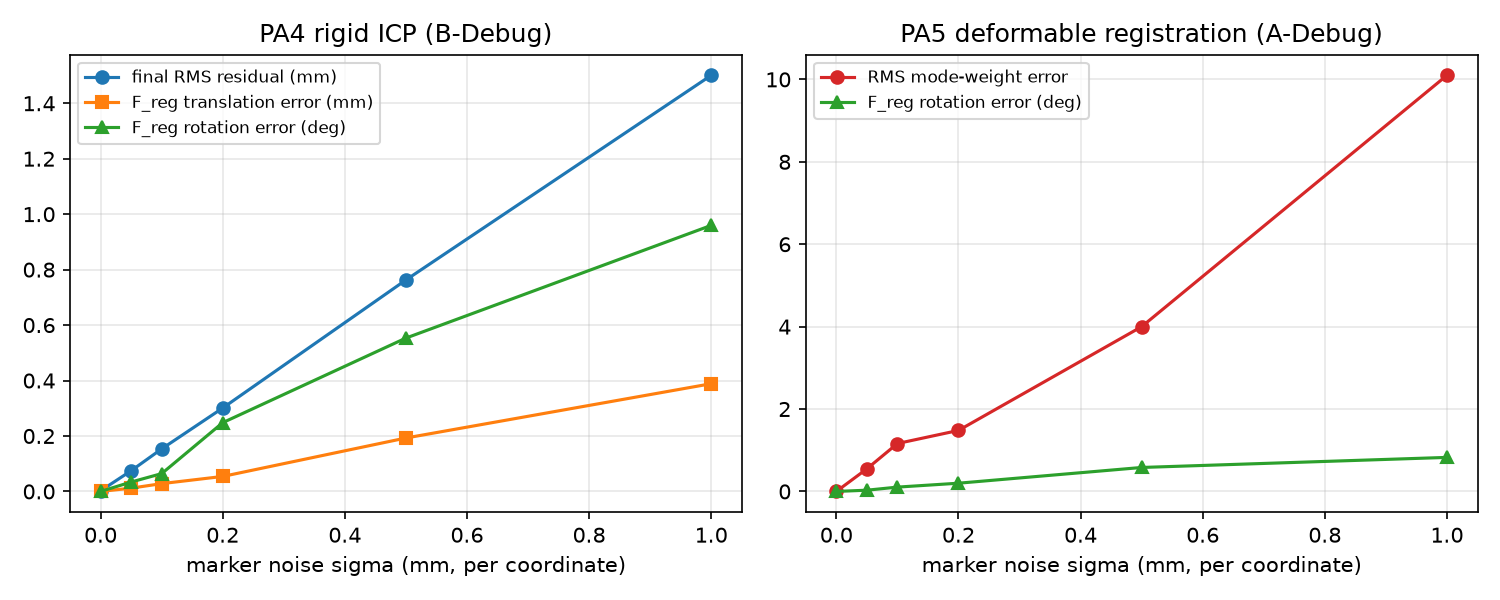
\includegraphics[width=0.49\textwidth]{marker_noise.png}
\caption{Left: share of ICP runs reaching the right minimum against the initial rotation error (and iterations needed). Right: errors against added marker noise for PA4 (rigid) and PA5 (deformable).}\label{fig:analysis}
\end{figure}

\paragraph{Discussion.} All three programs reproduce the instructor's debug results at the level permitted by the rounding of the data files, and their fits are at least as good as the instructor's in the least-squares sense. The main limitations are those of ICP itself: it needs an initial pose within roughly $75^\circ$, it converges linearly (tens to about a hundred iterations here), and it weights all pairs equally. The combined PA5 step converges faster than the alternation because it handles the coupling between pose and shape. Possible extensions are point-to-plane matching for faster convergence, a weighted or robust objective, and a prior on the mode weights (a penalty $\sum_m\lambda_m^2/\sigma_m^2$) to stabilize the weights when the data are noisy.

\paragraph{Statement of work.} This is an individual portfolio project by Parmida Mazloomi, carried out after the course and not submitted for credit. The problem, data and reference outputs are by R.~H.~Taylor and the CIS~I teaching staff; no code from other students' solutions was used.

\begin{thebibliography}{99}\small
\bibitem{handout34} R.~H.~Taylor, ``Programming Assignments 3 and 4,'' EN.601.455/655 Computer Integrated Surgery I, Johns Hopkins University, Fall 2025.
\bibitem{handout5} R.~H.~Taylor, ``Programming Assignment 5,'' EN.601.455/655, Fall 2025.
\bibitem{pa5notes} R.~H.~Taylor, ``Notes for PA5: Deformable registration to a statistical shape model,'' lecture notes, 2025.
\bibitem{lecframes} R.~H.~Taylor, ``Frames and frame transformations,'' CIS I lecture notes, 2025.
\bibitem{lecrigid} R.~H.~Taylor, ``Point cloud to point cloud rigid transformations,'' CIS I lecture notes.
\bibitem{lecpairs} R.~H.~Taylor, ``Finding point-pairs,'' CIS I lecture notes, 2010 to 2022.
\bibitem{lecreg1} R.~H.~Taylor, ``Registration, part 1'' (iterative closest point and outline of a practical ICP code), CIS I lecture notes, 2025.
\bibitem{arun} K.~S.~Arun, T.~S.~Huang and S.~D.~Blostein, ``Least-squares fitting of two 3-D point sets,'' \emph{IEEE Trans.\ PAMI}, 9(5):698-700, 1987.
\bibitem{umeyama} S.~Umeyama, ``Least-squares estimation of transformation parameters between two point patterns,'' \emph{IEEE Trans.\ PAMI}, 13(4):376-380, 1991.
\bibitem{besl} P.~J.~Besl and N.~D.~McKay, ``A method for registration of 3-D shapes,'' \emph{IEEE Trans.\ PAMI}, 14(2):239-256, 1992.
\bibitem{numpy} C.~R.~Harris et al., ``Array programming with NumPy,'' \emph{Nature}, 585:357-362, 2020.
\bibitem{lapack} E.~Anderson et al., \emph{LAPACK Users' Guide}, 3rd ed., SIAM, 1999.
\bibitem{matplotlib} J.~D.~Hunter, ``Matplotlib: a 2D graphics environment,'' \emph{Computing in Science \& Engineering}, 9(3):90-95, 2007.
\end{thebibliography}

\end{document}
